\chapter{DESENVOLVIMENTO DA SOLUÇÃO MOBILE}

O aplicativo foi desenvolvido com Flutter, \textit{framework} da Google que compila um único código em Dart para Android e iOS \cite{flutter2026}. A escolha considerou que os funcionários do armazém, da portaria e da frota usam celulares comuns, e que a câmera do aparelho pode substituir leitores de código de barras dedicados. A leitura usa a biblioteca \texttt{mobile\_scanner}, que reconhece tanto os códigos de barras das caixas e das notas quanto o QR Code impresso pelo Web para cada veículo.

\section{Telas principais e fluxo de navegação}

Após o login, o aplicativo mostra apenas as funções do perfil do usuário. A Figura~\ref{fig:navegacao} apresenta o fluxo de navegação: todas as telas de bipagem compartilham o mesmo leitor, que aceita a câmera ou a digitação do código.

\begin{figure}[htbp]
\centering
\caption{Fluxo de navegação do aplicativo}
\label{fig:navegacao}
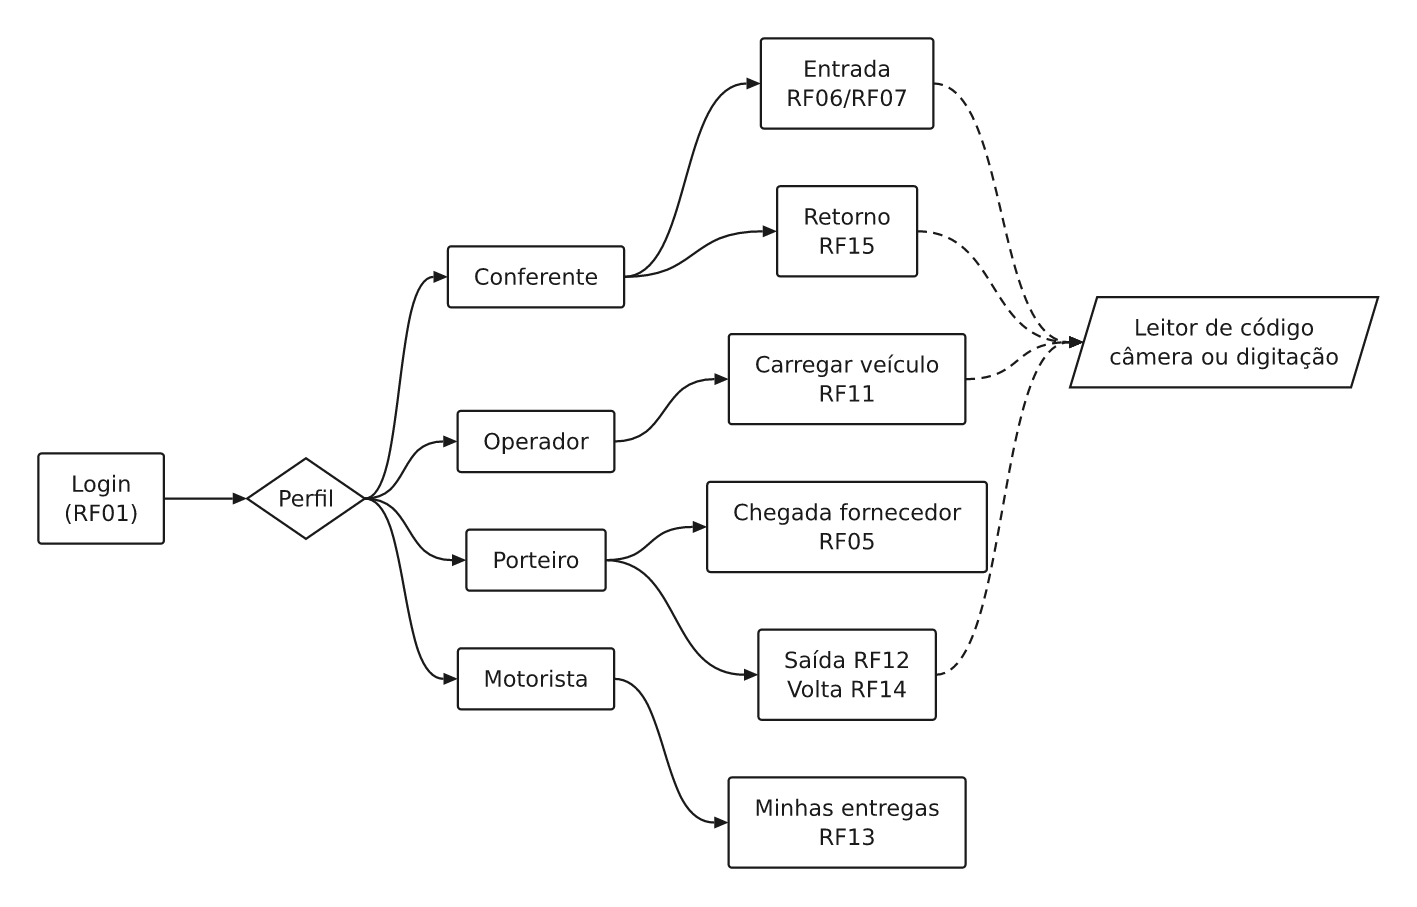
\includegraphics{figuras/navegacao_app.png}
\fonte{Elaborado pelo autor (2026)}
\end{figure}

A Figura~\ref{fig:app} mostra três telas do aplicativo executando no emulador Android com dados reais da API. Na tela do operador, o carregamento indica quantas caixas já subiram e o que ainda falta, pedido a pedido; a tela do motorista lista as entregas com cliente, endereço e botões de registro. Nas telas de bipagem, o leitor reabre automaticamente após cada leitura bem-sucedida e para no primeiro erro, para que a pessoa leia o motivo da recusa antes de continuar.

\begin{sidewaysfigure}
\centering
\caption{Telas do aplicativo: login, carregamento (operador) e entregas (motorista)}
\label{fig:app}
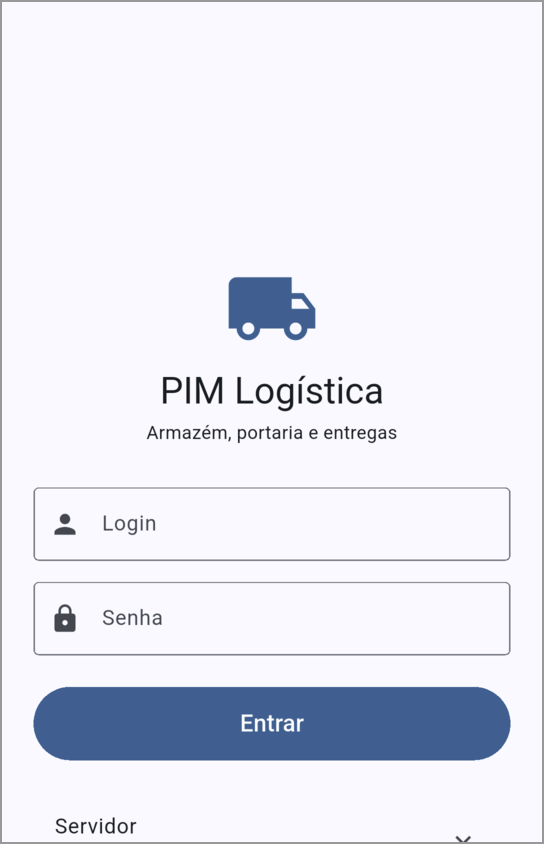
\includegraphics[height=12cm]{figuras/app_login.png}\hfill
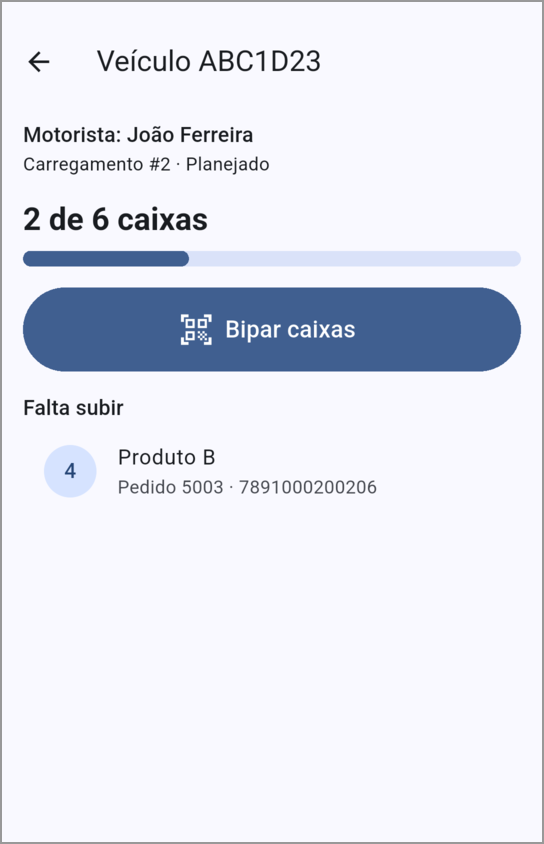
\includegraphics[height=12cm]{figuras/app_carregamento.png}\hfill
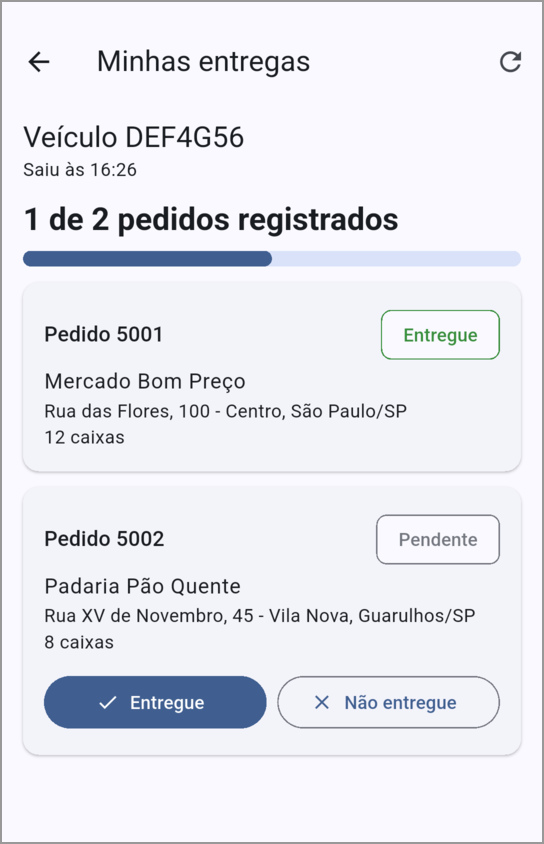
\includegraphics[height=12cm]{figuras/app_entregas.png}
\fonte{Elaborado pelo autor (2026)}
\end{sidewaysfigure}

\section{Autenticação e sincronização de dados}

No login, o aplicativo envia usuário e senha para \texttt{/auth/login} e guarda o token JWT, o nome e o perfil com a biblioteca \texttt{shared\_preferences}, de modo que o usuário não precisa entrar novamente a cada abertura. O endereço do servidor também é configurável na tela de login, o que permite usar o mesmo aplicativo no emulador e em aparelhos na rede da empresa. Quando a API responde \texttt{401}, sinal de token vencido ou inválido, a sessão é encerrada e o aplicativo volta automaticamente para o login.

A sincronização segue o modelo \textit{online}: cada leitura é enviada imediatamente à API, que valida a regra e grava no banco antes de responder. Assim, não existe estado divergente entre o celular e o servidor, e o Web enxerga cada bipagem no mesmo instante. As telas recarregam os dados após cada operação e oferecem a ação de ``puxar para atualizar''. Também é guardado no aparelho o identificador da entrada em andamento, permitindo que o conferente feche o aplicativo e continue a conferência depois. A limitação dessa escolha é a dependência de sinal; sem conexão, o aplicativo avisa o usuário e nada é gravado pela metade.

\section{Integração com as APIs}

A comunicação foi organizada em três camadas: \texttt{ApiClient}, que trata HTTP, token e erros; \texttt{PimApi}, com uma função por rota; e as classes de modelo, que convertem o JSON em objetos Dart. O código a seguir mostra como o cliente traduz as respostas de erro da API em uma exceção com a mensagem da regra, exibida ao usuário em vermelho e com vibração.

\begin{codeblock}[Tratamento das respostas da API, trecho simplificado (app/lib/api/api\_client.dart)]{Java}
if (resposta.statusCode >= 200 && resposta.statusCode < 300) return dados;
if (resposta.statusCode == 401) {
  aoPerderLogin?.call();   // volta para a tela de login
  throw ApiException(401, 'Sua sessao expirou. Entre de novo.');
}
if (resposta.statusCode == 403) {
  throw ApiException(403, 'Seu perfil nao tem acesso a esta funcao.');
}
// 400: mensagem da regra de negocio, ex.: "RN10: esta caixa nao pertence..."
throw ApiException(resposta.statusCode, dados['erro']);
\end{codeblock}
